\documentclass{article}
\usepackage{iclr2026_conference,times}
\input{math_commands.tex}
\usepackage{hyperref}
\usepackage{url}
\usepackage{amsmath,amssymb,amsthm}
\usepackage{booktabs}
\usepackage{graphicx}
\usepackage{multirow}
\usepackage{xcolor}

\newtheorem{theorem}{Theorem}
\newtheorem{proposition}{Proposition}
\newtheorem{lemma}{Lemma}
\newtheorem{corollary}{Corollary}
\newtheorem{remark}{Remark}
\newcommand{\todo}[1]{\textcolor{red}{[TODO: #1]}}
\newcommand{\crps}{\mathrm{CRPS}}

\title{Where Reinforcement Learning Belongs in Post-Training\\Time-Series Foundation Models}

% TODO: confirm author list, affiliations and order before submission.
\author{Vikram Kakaria \\
Princeton University \\
\texttt{vk5825@princeton.edu}
\And
Anish Kataria \\
\todo{affiliation} \\
\texttt{\todo{email}}
}

\newcommand{\fix}{\marginpar{FIX}}
\newcommand{\new}{\marginpar{NEW}}

\iclrfinalcopy % TODO: remove for anonymous submission

\begin{document}

\maketitle

\begin{abstract}
Reinforcement learning (RL) post-training transformed language models, and the first RL recipes for time-series foundation models (TSFMs) have followed the same template: sample forecasts from the model's predictive distribution, reward them by point error, and apply GRPO. We show that this template is ill-posed for a probabilistic forecaster. Any per-sample reward, including a proper scoring rule applied sample by sample, defines an objective that is linear in the predictive distribution and is therefore maximised at a point mass; with a KL penalty the optimum is a tempered reference, still narrower under any point reward. Empirically, every published recipe (TS-GRPO, GTN-R, TimeRFT- and TPO-style training) buys a small point-error gain by shrinking uncertainty: on TimesFM-3, Chronos-T5 and Chronos-Bolt, 80\% coverage falls from nominal to 0.55--0.73, and to 0.24 with per-step credit, while supervised fine-tuning with the model's own proper loss improves every metric and keeps calibration. A set-level proper reward removes the collapse only for models that genuinely sample (token samplers), and on quantile heads the differentiable loss dominates. We then place RL where it is well-posed: a small agent that chooses the context a frozen oracle is shown and how much to trust it, delivering a linear pool of the oracle's forecast with a calibrated fallback, rewarded by a proper score of the \emph{delivered} distribution. We prove that this agent cannot be rewarded for overconfidence, that it has $O(\sqrt{T\log K})$ regret against the best fixed context, that pooling never hurts in expectation, and that decision costs with a randomised critical fractile are themselves proper rewards. We release a single implementation covering four oracle families, walk-forward evaluation with paired-bootstrap intervals and calibration tests, and report \todo{the agent's results on GIFT-Eval and fev-bench covariate tasks}.
\end{abstract}

\section{Introduction}
Time-series foundation models (TSFMs) such as TimesFM \citep{das2023timesfm}, Chronos \citep{ansari2024chronos,ansari2025chronos2}, Moirai \citep{woo2024moirai}, TiRex \citep{auer2025tirex} and Toto \citep{cohen2025toto} are strong zero-shot probabilistic forecasters, and they are well calibrated out of the box \citep{adler2026calibrated}. The natural next question, by analogy with language models, is how to post-train them for a user's data. The first answers \citep{qi2025timehf,li2026timerft,zhang2026gtnr} copy the language-model recipe: sample trajectories from the model's predictive distribution, score each by a point error, and update with GRPO \citep{shao2024deepseekmath}. All of them report mean-squared or mean-absolute error and none reports a probabilistic metric or calibration; the field's own survey of TSFM post-training cites no RL work at all \citep{xie2026survey}.

This paper asks where RL belongs in post-training a probabilistic forecaster, and answers in three parts.

\textbf{An audit with a theorem.} Section~\ref{sec:collapse} shows that the sampled-trajectory recipe is ill-posed: the policy-gradient objective is linear in the predictive distribution, so its optimum is a point mass whatever the reward (Proposition~\ref{prop:linear}), a KL penalty only tempers the reference (Proposition~\ref{prop:kl}), and a proper scoring rule applied to one sample at a time is not proper (Proposition~\ref{prop:persample}). On three model families the recipe drops 80\% coverage from nominal to 0.55--0.73 while supervised fine-tuning (SFT) with the model's own proper loss improves accuracy and keeps calibration (Section~\ref{sec:audit}). A set-level proper reward is consistent (Proposition~\ref{prop:set}) and preserves calibration on a token sampler, but not on a quantile head, where the sampling step is a device (Remark~\ref{rem:device}).

\textbf{An agent around a frozen oracle.} Section~\ref{sec:agent} places RL on the choices around the forecaster instead of inside it: which context the oracle is shown and how much to trust it. The delivered forecast is a linear pool of the oracle's forecast under the chosen context with a calibrated fallback; the reward is a proper score of the delivered distribution. We prove calibration by construction (Theorem~\ref{thm:calib}), a regret bound against the best fixed context (Theorem~\ref{thm:regret}), that pooling never hurts in expectation (Proposition~\ref{prop:pool}), and that a newsvendor cost with a uniformly randomised critical fractile is itself a proper reward (Proposition~\ref{prop:utility}). Because every action can be scored once the outcome is observed, the policy objective is computed exactly (full-information policy optimisation), and RL is reserved for the discrete, sequential and decision-valued parts of the problem where supervised learning does not apply.

\textbf{A protocol and an implementation.} Section~\ref{sec:protocol} fixes an evaluation protocol with no free thresholds: walk-forward folds, paired-bootstrap intervals over held-out windows, binomial-coverage and PIT-uniformity tests on every arm, and hidden-test discipline on public leaderboards \citep{aksu2024gifteval,shchur2025fevbench}. One implementation covers TimesFM-3, Chronos-2, Chronos-Bolt and Chronos-T5 behind a common interface, so every trainer, reward and test runs unchanged across oracles. \todo{Section~\ref{sec:results-agent} reports the agent on electricity, ETT and the leaderboard covariate tasks, with transfer across oracles.}

Our closest neighbour is PostTime \citep{liu2026posttime}, which post-trains a 4B language model to revise a frozen TimesFM-2.5 forecast from text context with SFT followed by RL on an improvement-ratio reward. We share the two-stage recipe and the frozen prior; we differ in the object (a numeric agent over context and trust), in the reward (a proper score of the delivered distribution rather than a point error), in the guarantees, in what is measured (calibration, regret, utility), and in showing the same agent across several oracles.

\section{Related work}
\paragraph{RL post-training of TSFMs.} TimeHF \citep{qi2025timehf} wraps a point model as a Gaussian and applies a REINFORCE-style objective to human-labelled preference pairs. TimeRFT \citep{li2026timerft} applies GRPO to patch-level samples from Moirai-MoE, Chronos-2 and Toto with an exponential-error reward and per-step credit. TS-GRPO and its ground-truth-neighbourhood regulariser GTN-R \citep{zhang2026gtnr} apply GRPO with an MSE reward and document a ``suboptimal collapse'' of probability mass, which they regularise; calibration is not measured. PostTime \citep{liu2026posttime} trains a language-model reviser over a frozen TSFM. All report point metrics only. Supervised adaptation is better studied: LoRA \citep{hu2022lora,gupta2024lora}, in-context fine-tuning \citep{das2025icf}, and a systematic fine-tuning study that finds full fine-tuning can hurt and LoRA can sharpen the median at the cost of the predictive distribution \citep{laglil2026finetuning}.

\paragraph{RL for language models and calibration.} Verifiable-reward RL \citep{deepseek2025r1,lambert2024tulu3} reweights what the base model can already produce \citep{yue2025does}; entropy collapse has a closed form \citep{cui2025entropy}; GRPO's group-standard-deviation normalisation biases the update \citep{liu2025drgrpo} and, on stochastic outcomes, induces overconfidence that leave-one-out baselines avoid \citep{turtel2025outcome,bereket2025uncalibrated,ahmadian2024rloo}; even random rewards move a model \citep{shao2025spurious}. Rewards that are proper in a \emph{reported} probability have calibrated optima \citep{damani2025rlcr}, and set-level rewards over sampled rollouts have been proposed for regression \citep{park2026distaware}. We transfer these results to forecasters and show which of them survive the change of object.

\paragraph{Context, retrieval and combination for frozen forecasters.} Test-time search over context transformations moves error by 13--65\% \citep{qiu2026tato}; retrieval mixers \citep{ning2025tsrag} and online weighters \citep{lee2025elf,das2025synapse} are supervised; retrieval policies for language models are trained by RL \citep{hsu2024leret,jin2025searchr1}. Forecast combination has a long theory: linear pools \citep{ranjan2010combining}, quantile averaging \citep{lichtendahl2013quantile}, online aggregation with regret bounds \citep{cesabianchi2006prediction,berrisch2021crps}. Decision-focused learning \citep{elmachtoub2022smart} has been applied once to a TSFM \citep{beichter2025dfl}; CRPS-optimal combinations need not be profit-optimal \citep{nitka2023combining}.

\section{Preliminaries}
A forecaster maps a context (history $x_{1:T}$ and optional covariate rows $Z$) to a predictive distribution $p$ over the future $y_{1:H}$. The models we study report $p$ through $Q$ quantiles at levels $\tau_1<\dots<\tau_Q$ (TimesFM-3, Chronos-Bolt, Chronos-2) or through a categorical distribution over value bins sampled autoregressively (Chronos-T5). The continuous ranked probability score is
\begin{equation}
\crps(p, y) = \E_{X\sim p}|X-y| - \tfrac12\,\E_{X,X'\sim p}|X-X'| = 2\int_0^1 \rho_\tau\big(y - q_\tau(p)\big)\,d\tau,
\label{eq:crps}
\end{equation}
where $\rho_\tau(u)=u(\tau-\mathbf{1}[u<0])$ is the pinball loss; it is strictly proper \citep{gneiting2007strictly}, and on a quantile grid it is approximated by twice the mean pinball loss. A scoring rule $S(p,y)$ is proper if $\E_{y\sim p^*}S(p^*,y)\le\E_{y\sim p^*}S(p,y)$ for all $p$, with equality only at $p=p^*$ when strictly proper. Group-relative policy optimisation (GRPO) samples $K$ trajectories $\tau_k\sim p_\theta$ per context, computes rewards $r_k$, advantages $A_k=(r_k-\bar r)/(\sigma_r+\epsilon)$, and ascends $\sum_k A_k\nabla_\theta\log p_\theta(\tau_k)$ with a KL penalty to a reference.

\section{Why RL on the predictive distribution collapses}
\label{sec:collapse}
Let $\mathcal{P}$ be the set of predictive distributions the forecaster can express and $r:\mathcal{Y}\to\mathbb{R}$ a reward on trajectories. The sampled-trajectory objective is $J(p)=\E_{\tau\sim p}[r(\tau)]$.

\begin{proposition}[Point-mass optimum]
\label{prop:linear}
$J$ is linear in $p$. If $\mathcal{P}$ contains the point masses, $\sup_{p\in\mathcal{P}}J(p)$ is attained at a Dirac at $\arg\max_\tau r(\tau)$; in particular no per-trajectory reward has a non-degenerate maximiser.
\end{proposition}

\begin{proposition}[KL tempering]
\label{prop:kl}
For $J_\beta(p)=\E_{\tau\sim p}[r(\tau)]-\beta\,\mathrm{KL}(p\,\|\,p_{\mathrm{ref}})$, the maximiser is $p^\star(\tau)\propto p_{\mathrm{ref}}(\tau)\exp(r(\tau)/\beta)$ \citep{korbak2022rl}. If $r$ is a decreasing function of the distance to a fixed target, $p^\star$ is a tempering of $p_{\mathrm{ref}}$ toward that target and is strictly narrower than $p_{\mathrm{ref}}$ for every $\beta<\infty$.
\end{proposition}

\begin{proposition}[Per-sample proper scores are not proper]
\label{prop:persample}
Let $r(\tau)=-\crps(\delta_\tau,y)=-|\tau-y|$ be the CRPS of the degenerate distribution at the sample. Then $\E_{\tau\sim p}[r(\tau)]=-\E_{\tau\sim p}|\tau-y|$, which drops the spread term $\tfrac12\E|X-X'|$ of \eqref{eq:crps}; its maximiser over $p$ is the point mass at $y$ in hindsight and the conditional median in expectation. The same holds for any proper score applied to single samples.
\end{proposition}

\begin{proposition}[Set-level proper rewards are consistent]
\label{prop:set}
Let $R_K(\tau_{1:K},y)=-\widehat{\crps}_K(\tau_{1:K},y)$ be the fair (unbiased) sample estimator of $-\crps(p,y)$ from $K\ge2$ i.i.d. draws. Then $\E_{\tau_{1:K}\sim p}[R_K]=-\crps(p,y)$ exactly, so the expected set-level reward is a strictly proper score of $p$ and its unique maximiser in expectation over $y\sim p^*$ is $p=p^*$.
\end{proposition}

\begin{remark}[Entropy dynamics and the advantage normaliser]
Under any policy gradient the change in entropy is proportional to $-\mathrm{Cov}_{\tau\sim p}(\log p(\tau), A(\tau))$ \citep{cui2025entropy}; a reward that favours samples near the model's own mode makes this covariance positive and entropy fall. Dividing advantages by the within-group standard deviation removes the asymmetry a proper score assigns to confident misses and, for a forecaster, normalises away the predictive spread itself \citep{turtel2025outcome,bereket2025uncalibrated}.
\end{remark}

\begin{remark}[Quantile heads: the sampling step is a device]
\label{rem:device}
For a deterministic quantile head, ``sampling'' means inverse-CDF draws through a piecewise-linear density fitted to the quantiles, with $u$ clipped away from the tails; the score-function identity $\E_{\tau\sim p_\theta}[\nabla_\theta\log p_\theta(\tau)]=0$ does not hold for such a device, so even a set-level reward produces a biased, sharpening update. Proposition~\ref{prop:set} applies to models that genuinely sample; for quantile heads the differentiable proper loss is the correct object and, as Section~\ref{sec:audit} shows, the better one.
\end{remark}
Proofs are in Appendix~\ref{app:proofs}.

\section{An agent around a frozen oracle}
\label{sec:agent}
\paragraph{Setup.} An episode is $(x_{1:T}, Z, y_{1:H})$. The oracle $f$ is frozen and maps a \emph{context} $c$ (a subset of candidate rows $Z_c$ as past-only or known-future covariates, a history length, optional transforms) to a quantile forecast $p_c=f(x,Z_c)$. A calibrated fallback $p_0$ is a seasonal-naive point forecast with per-horizon residual quantiles estimated by rolling origins inside the history (Appendix~\ref{app:impl}). The agent observes $s=\phi(x,Z,\mathrm{diag}(f))$, where the diagnostics are the width of $f$'s band, the disagreement of its median across candidate contexts, and its width relative to the fallback, and selects an action $a=(c,w)$ with $c\in\{1,\dots,K\}$ and $w$ on a grid in $[0,1]$. The delivered forecast is the linear pool
\begin{equation}
p_a = w\,p_c + (1-w)\,p_0,
\label{eq:pool}
\end{equation}
whose quantiles are obtained by inverting the pooled CDF. The reward is $r(a)=-\crps(p_a,y)$, or PostTime's improvement ratio $\mathrm{clip}_{[0,1]}\big(\tfrac12+\tfrac12(1-\crps(p_a,y)/\crps(p_{\mathrm{native}},y))\big)$, or a decision cost (Proposition~\ref{prop:utility}).

\paragraph{Training.} \emph{Stage 1 (hindsight supervision).} Because $y$ is observed after the fact, every action is scored, $a^\star=\arg\max_a r(a)$ is the label, and windows where the native context with $w=1$ wins are fallback examples by construction (the analogue of PostTime's verified-trace construction with the ground truth as the verifier). \emph{Stage 2 (full-information policy optimisation).} With all $r(a)$ known, the policy objective $\E_{a\sim\pi_\theta(\cdot|s)}[r(a)-r(a_{\mathrm{native}})]$ is computed exactly over the action set and ascended directly, with an entropy bonus; sampled GRPO with a leave-one-out baseline is used only when the action set is too large to enumerate. The oracle receives no gradient in either stage.

\begin{theorem}[Calibration by construction]
\label{thm:calib}
Let $r(a)=S(p_a,y)$ with $S$ strictly proper, and let the agent control $p_a$ only through \eqref{eq:pool}. Then for every state, $\E_{y\sim p^*}[r(a)]$ is maximised by the action whose delivered distribution is closest to $p^*$ in the divergence induced by $S$; no action is rewarded for reducing the spread of $p_a$ below that of $p^*$. In particular, no action edits the oracle's quantiles, so the oracle's calibration is preserved under $w=1$ and the fallback's under $w=0$.
\end{theorem}

\begin{theorem}[Regret against the best fixed context]
\label{thm:regret}
Consider $T$ episodes, $A=K|W|$ actions, and losses $\ell_t(a)=\crps(p_{a,t},y_t)\in[0,L]$. Since every $\ell_t(a)$ is observed after $y_t$, exponentially weighted averaging over actions with rate $\eta=\sqrt{8\log A/T}/L$ attains $\sum_t\E_{a\sim\pi_t}\ell_t(a)-\min_a\sum_t\ell_t(a)\le L\sqrt{(T/2)\log A}$ \citep{cesabianchi2006prediction}. Quantile-wise aggregation under CRPS attains faster rates \citep{berrisch2021crps}.
\end{theorem}

\begin{proposition}[Pooling never hurts in expectation]
\label{prop:pool}
$\crps(\cdot,y)$ is convex in the distribution, so $\crps(w p_c+(1-w)p_0,y)\le w\,\crps(p_c,y)+(1-w)\crps(p_0,y)$ for all $w\in[0,1]$; the expected-CRPS-optimal $w$ is at least as good as either component \citep{ranjan2010combining}.
\end{proposition}

\begin{proposition}[Utility-proper decision environments]
\label{prop:utility}
For the newsvendor decision $d_\tau(p)=q_\tau(p)$ with critical fractile $\tau$ and cost $c_\tau(d,y)=\rho_\tau(y-d)$, the expected cost with $\tau\sim\mathrm{Unif}(0,1)$ equals $\tfrac12\crps(p,y)$ by \eqref{eq:crps}. Hence a decision reward with a uniformly randomised critical fractile is a strictly proper score and inherits Theorem~\ref{thm:calib}. The same construction applies to CVaR levels in position sizing.
\end{proposition}

\paragraph{Where RL is needed.} The trust weight alone is a continuous parameter of a differentiable objective and could be fit by supervised CRPS minimisation. RL earns its place for the discrete context choice, for sequential settings in which the agent decides when to refresh or re-anchor as data arrives, and for decision rewards that are not differentiable. The design uses the proper score everywhere and RL only there.

\section{Evaluation protocol}
\label{sec:protocol}
\textbf{Walk-forward.} Every real-data result uses rolling forecast origins: at each origin, training windows end before the origin (with a gap of one window) and held-out windows follow it; every fold restarts from the released model; results are pooled over origins. \textbf{Intervals.} Frozen and post-trained forecasts are paired per held-out window and the change is bootstrapped over windows (4{,}000 resamples); an effect is reported only with its interval. \textbf{Calibration.} There are no tolerances: an arm ``keeps calibration'' if the interval on its coverage change includes zero and it passes the same binomial test of 80\% coverage against nominal and Kolmogorov--Smirnov test of PIT uniformity that the frozen model passes. \textbf{Arms.} One per claim: oracle with native context; best fixed context in hindsight on training windows (the regret reference); SFT of the oracle with its proper loss; SFT-agent; SFT+RL agent; RL agent with a random reward (control); a supervised non-foundation model trained on the training windows. \textbf{Transfer.} An agent trained on one oracle is evaluated unchanged on the others. \textbf{Hidden tests.} Training uses only GIFT-Eval train splits, fev-bench training windows and Time-Series-Library data; leaderboard test splits are scored once through the official harnesses. \textbf{Counts.} Origins are set by series length with blocks at least one horizon apart; seeds and windows per origin by a power calculation against the pilot's window-level variance (Appendix~\ref{app:power}).

\section{Results}
\subsection{Audit: the sampled-trajectory recipe on three model families}
\label{sec:audit}
\textbf{TimesFM-3.} We attach LoRA ($r{=}8$) to the variate-attention projections of layers 10--14 of the frozen 331M model and run 300 steps of each method on a synthetic bank of covariate laws with known conditional means and on hourly electricity load, scoring 128 held-out windows (Table~\ref{tab:audit-tfm}; Figure~\ref{fig:synth}). Every method improves point accuracy on the synthetic bank; SFT with the pinball loss improves most and keeps coverage near nominal; every sampled-trajectory method narrows the interval below nominal, and the three GRPO rewards (MSE, per-sample CRPS, composite) are indistinguishable, as Propositions~\ref{prop:linear}--\ref{prop:persample} predict. Per-step credit collapses coverage to 0.24 and PPO diverges. On electricity, nothing moves at this budget.

\begin{table}[t]
\caption{TimesFM-3, synthetic laws, 300 CPU steps, 128 held-out windows, frozen $\to$ post-trained with paired-bootstrap 95\% intervals on the change. Bold: interval excludes zero.}
\label{tab:audit-tfm}
\centering\small
\begin{tabular}{lccc}
\toprule
cell & MASE & CRPS & 80\% coverage \\
\midrule
frozen & 1.142 & 0.465 & 0.82 \\
SFT, pinball (M1) & \textbf{1.067} $(-0.107,-0.045)$ & \textbf{0.439} $(-0.035,-0.017)$ & 0.78 \\
GRPO, $-$MSE, std (TS-GRPO, M2) & \textbf{1.107} $(-0.053,-0.019)$ & \textbf{0.456} $(-0.013,-0.004)$ & \textbf{0.73} \\
+ ground-truth anchor (GTN-R, M3) & \textbf{1.088} $(-0.080,-0.031)$ & \textbf{0.451} $(-0.021,-0.007)$ & \textbf{0.70} \\
per-step credit (TimeRFT-like, M4) & \textbf{1.103} $(-0.067,-0.012)$ & \textbf{0.518} $(+0.041,+0.064)$ & \textbf{0.24} \\
trajectory preference, IPO (TPO-like, M5) & \textbf{1.101} $(-0.061,-0.023)$ & \textbf{0.454} $(-0.017,-0.005)$ & \textbf{0.71} \\
PPO, composite (M6) & \textbf{1.256} $(+0.082,+0.147)$ & \textbf{0.615} $(+0.137,+0.165)$ & \textbf{0.11} \\
GRPO, per-sample CRPS & \textbf{1.110} $(-0.049,-0.017)$ & \textbf{0.457} $(-0.012,-0.003)$ & \textbf{0.72} \\
GRPO, composite (M7) & \textbf{1.109} $(-0.050,-0.018)$ & \textbf{0.456} $(-0.013,-0.004)$ & \textbf{0.73} \\
\midrule
\multicolumn{4}{l}{\emph{Electricity (321 clients), same protocol:} frozen MASE 1.376, CRPS 0.237, coverage 0.79;} \\
\multicolumn{4}{l}{SFT 1.389 / 0.240 / 0.80; GRPO $-$MSE 1.374 / 0.237 / 0.78; GRPO composite 1.371 / 0.237 / 0.77; all intervals include zero.} \\
\bottomrule
\end{tabular}
\end{table}

\begin{figure}[t]
\centering
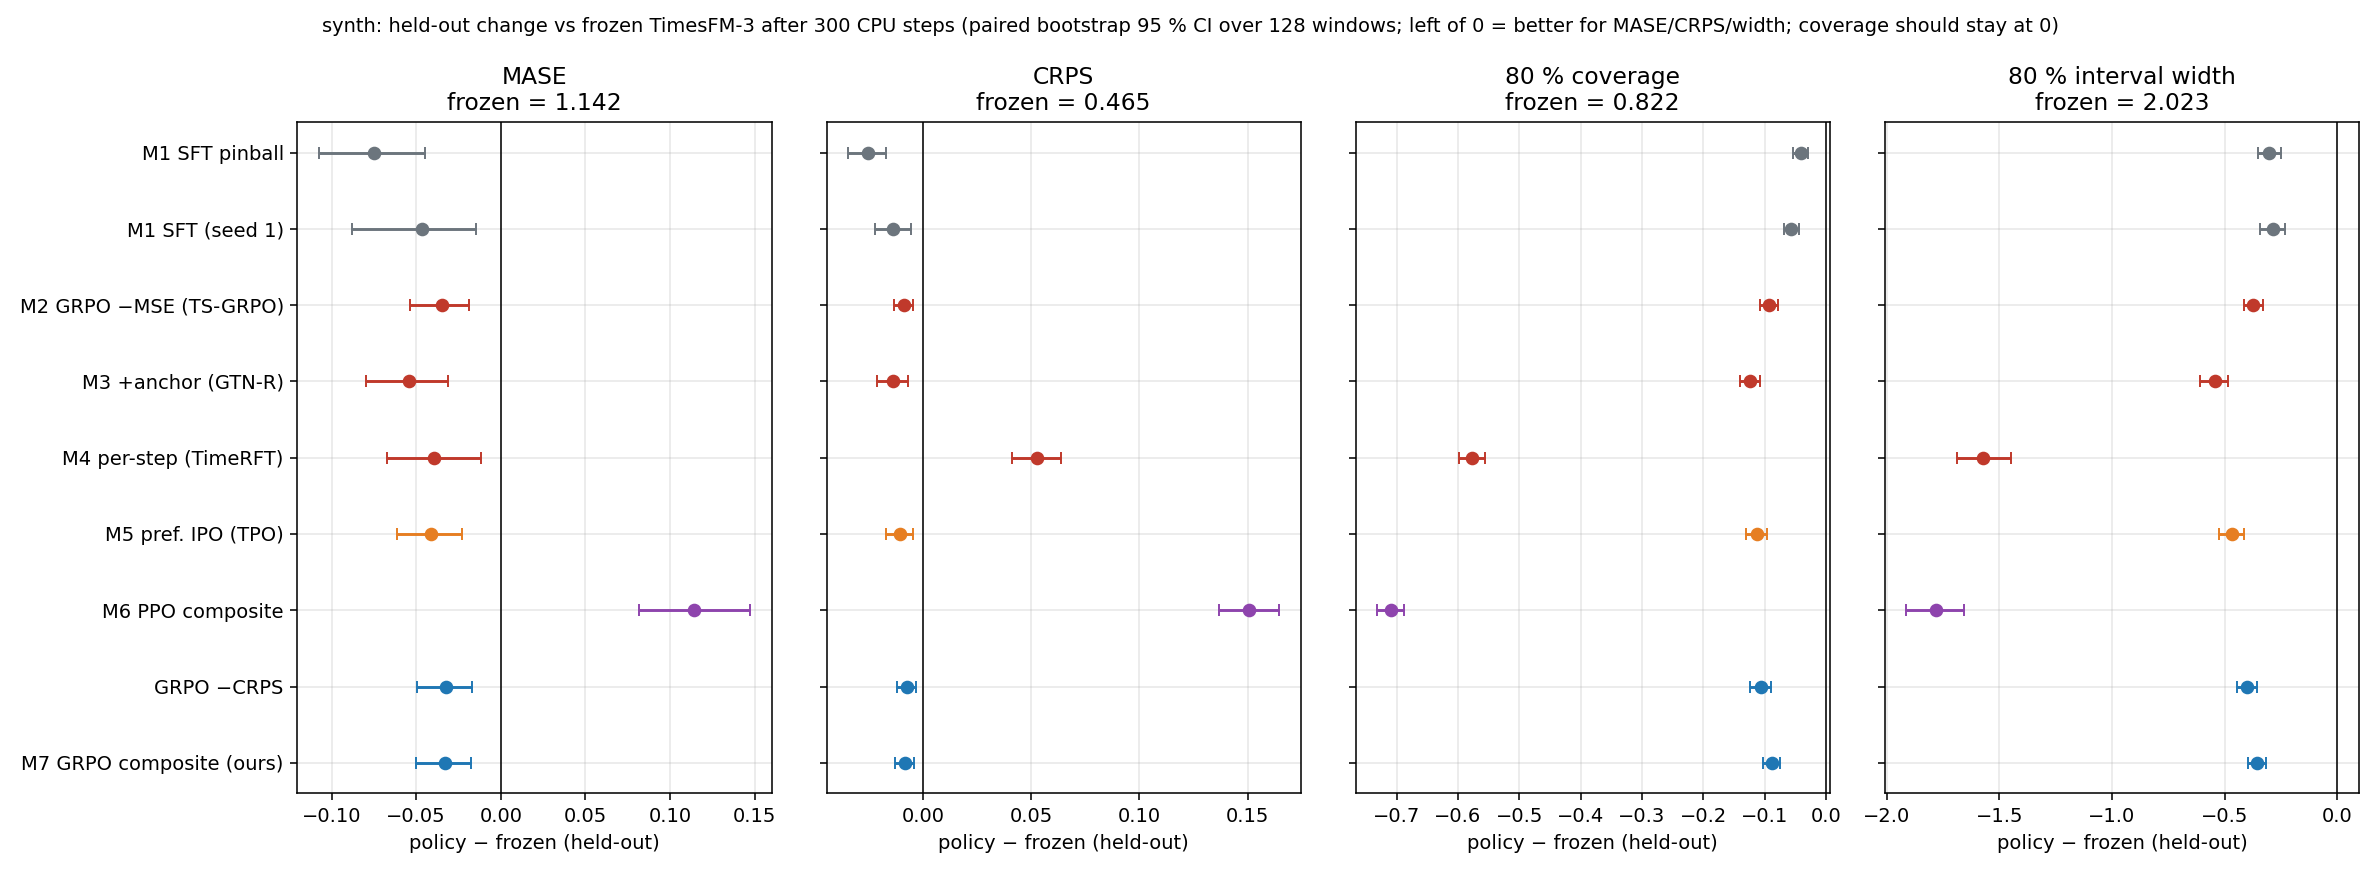
\includegraphics[width=\linewidth]{figures/synth_deltas.png}
\caption{TimesFM-3, synthetic bank: change from the frozen model per cell with 95\% paired-bootstrap intervals. Left of zero is better for MASE, CRPS and width; coverage should stay at zero. Every sampled-trajectory method trades coverage for point error; the three GRPO rewards coincide.}
\label{fig:synth}
\end{figure}

\textbf{Chronos-T5 and Chronos-Bolt.} To separate the reward from the model type we repeat the comparison on a token sampler (Chronos-T5-tiny) and a quantile head (Chronos-Bolt-tiny) with the same code, on ETTh1 under a chronological split (Table~\ref{tab:pilot}). The literature recipe drops coverage by nine and ten points on both. Removing the standard-deviation normalisation halves the loss on both and gives the only significant RL accuracy gain on the sampler. The set-level fair-CRPS reward keeps the sampler calibrated (coverage change $+0.009$, interval on zero) and collapses the quantile head exactly like MSE ($-0.103$), as Remark~\ref{rem:device} predicts. SFT is the only cell that improves both MASE and CRPS significantly on the quantile head with coverage intact.

\begin{table}[t]
\caption{Pilot on two Chronos families, ETTh1, chronological split, 150 steps, one seed; change from frozen with 95\% paired-bootstrap intervals. Chronos-T5 intervals are wide because its score is itself a 20-sample estimate.}
\label{tab:pilot}
\centering\small
\begin{tabular}{llccc}
\toprule
model & cell & $\Delta$MASE & $\Delta$CRPS & $\Delta$coverage \\
\midrule
\multirow{4}{*}{Bolt (quantile head)} & SFT, pinball & $\mathbf{-0.012}$ $(-0.022,-0.002)$ & $\mathbf{-0.003}$ $(-0.005,-0.002)$ & $-0.001$ \\
 & GRPO, $-$MSE, std & $-0.013$ $(-0.032,+0.005)$ & $\mathbf{+0.008}$ $(+0.003,+0.013)$ & $\mathbf{-0.099}$ \\
 & GRPO, $-$MSE, LOO & $-0.013$ $(-0.028,+0.000)$ & $+0.002$ $(-0.001,+0.005)$ & $\mathbf{-0.046}$ \\
 & GRPO, set-level CRPS & $-0.011$ $(-0.031,+0.006)$ & $\mathbf{+0.010}$ $(+0.005,+0.014)$ & $\mathbf{-0.103}$ \\
\midrule
\multirow{4}{*}{T5 (token sampler)} & SFT, cross-entropy & $-0.007$ $(-0.068,+0.055)$ & $-0.008$ $(-0.023,+0.009)$ & $\mathbf{+0.048}$ \\
 & GRPO, $-$MSE, std & $-0.035$ $(-0.128,+0.053)$ & $+0.003$ $(-0.019,+0.025)$ & $\mathbf{-0.088}$ \\
 & GRPO, $-$MSE, LOO & $\mathbf{-0.095}$ $(-0.180,-0.023)$ & $-0.017$ $(-0.036,+0.001)$ & $-0.014$ \\
 & GRPO, set-level CRPS & $+0.001$ $(-0.062,+0.065)$ & $-0.007$ $(-0.026,+0.010)$ & $+0.009$ \\
\bottomrule
\end{tabular}
\end{table}

\subsection{The agent}
\label{sec:results-agent}
\todo{Walk-forward results of the agent arms on electricity and ETT with TimesFM-3 and Chronos-2 as oracles: CRPS skill vs oracle with intervals, coverage change with intervals, calibration tests, regret vs best fixed context, the random-reward control, and transfer of the TimesFM-3-trained agent to Chronos-2, Chronos-Bolt and Chronos-T5. Table~\ref{tab:agent} is the planned layout.}

\begin{table}[t]
\caption{Planned layout: agent arms, walk-forward, pooled over origins, three seeds. \todo{fill from runs/agent}}
\label{tab:agent}
\centering\small
\begin{tabular}{lcccc}
\toprule
arm & CRPS skill vs oracle (95\% CI) & $\Delta$coverage (95\% CI) & calibration tests & regret vs best fixed \\
\midrule
oracle, native context & 0 & 0 & \todo{} & \todo{} \\
best fixed context & \todo{} & \todo{} & \todo{} & 0 \\
SFT-CRPS of the oracle & \todo{} & \todo{} & \todo{} & \todo{} \\
SFT-agent & \todo{} & \todo{} & \todo{} & \todo{} \\
SFT+RL agent & \todo{} & \todo{} & \todo{} & \todo{} \\
RL agent, random reward & \todo{} & \todo{} & \todo{} & \todo{} \\
supervised PatchTST & \todo{} & \todo{} & \todo{} & --- \\
\bottomrule
\end{tabular}
\end{table}

\subsection{Leaderboards and decisions}
\todo{GIFT-Eval and fev-bench covariate tasks through the official harnesses, tagged fine-tuned; newsvendor and execution environments with the randomised-fractile reward (Proposition~\ref{prop:utility}); utility with intervals and the calibration of the intervals that drove the decisions.}

\section{Limitations}
The audit is at small scale (hundreds of steps, one seed, tiny Chronos checkpoints) and its magnitudes will change at scale even though the mechanism does not depend on the budget. The agent's gains depend on the presence of useful context; on univariate leaderboard tasks with no covariates the context action reduces to history length and transforms. Our fallback is deliberately simple; a stronger fallback shifts credit from the oracle to the pool. Decision environments use public cost models, not a firm's.

\section{Conclusion}
RL post-training of a probabilistic forecaster is ill-posed when the policy is the forecaster's own predictive distribution: the objective is linear in the distribution and its optimum is a point mass, which is what every published recipe exhibits as a loss of calibration. It is well-posed when the policy acts on what a frozen oracle is shown and how much it is trusted, with a proper score of the delivered distribution as the reward, where it comes with calibration, regret and decision guarantees. \todo{The agent's empirical gains on public benchmarks decide how much this buys in practice.}

\bibliography{refs}
\bibliographystyle{iclr2026_conference}

\appendix
\section{Proofs}
\label{app:proofs}
\begin{proof}[Proof of Proposition~\ref{prop:linear}]
$J(p)=\int r\,dp$ is a linear functional of the measure $p$. The set of probability measures on $\mathcal{Y}$ is convex with the point masses as its extreme points, and a linear functional on a convex set attains its supremum at an extreme point. If $\mathcal{P}$ contains the point masses, $\sup J=\sup_\tau r(\tau)$, attained at $\delta_{\tau^\star}$. If $\mathcal{P}$ is a parametric family that does not contain point masses, the supremum is approached along sequences whose spread vanishes wherever the family allows it.
\end{proof}
\begin{proof}[Proof of Proposition~\ref{prop:kl}]
Adding the Lagrangian of the normalisation constraint and setting the first variation of $\int r\,dp-\beta\int p\log(p/p_{\mathrm{ref}})$ to zero gives $r-\beta(\log p-\log p_{\mathrm{ref}}+1)-\lambda=0$, i.e.\ $p\propto p_{\mathrm{ref}}e^{r/\beta}$ \citep{korbak2022rl}. If $r(\tau)=-g(|\tau-y_0|)$ with $g$ increasing, the tilt $e^{r/\beta}$ is a decreasing function of $|\tau-y_0|$, so $p^\star$ is $p_{\mathrm{ref}}$ reweighted toward $y_0$; its variance is strictly smaller than that of $p_{\mathrm{ref}}$ unless $p_{\mathrm{ref}}$ is degenerate, since multiplying a density by a unimodal weight centred at $y_0$ reduces spread around $y_0$ and the reweighted mean moves toward $y_0$.
\end{proof}
\begin{proof}[Proof of Proposition~\ref{prop:persample}]
$\crps(\delta_\tau,y)=\E|X-y|-\tfrac12\E|X-X'|$ with $X,X'\sim\delta_\tau$ equals $|\tau-y|-0$. Hence $\E_{\tau\sim p}[-\crps(\delta_\tau,y)]=-\E_{\tau\sim p}|\tau-y|$, which is $-\crps(p,y)-\tfrac12\E_{X,X'\sim p}|X-X'|$: the sampled-trajectory objective equals the proper score minus the spread term, and is maximised by concentrating $p$ at the minimiser of $\E|\tau-y|$. For a general proper score $S$, $\E_{\tau\sim p}S(\delta_\tau,y)$ is linear in $p$ and Proposition~\ref{prop:linear} applies.
\end{proof}
\begin{proof}[Proof of Proposition~\ref{prop:set}]
The fair estimator $\widehat{\crps}_K=\frac1K\sum_k|\tau_k-y|-\frac{1}{2K(K-1)}\sum_{k\ne k'}|\tau_k-\tau_{k'}|$ has expectation $\E|X-y|-\tfrac12\E|X-X'|=\crps(p,y)$ under i.i.d.\ sampling. Therefore $\E_{\tau_{1:K}\sim p}[R_K]=-\crps(p,y)$, and $\E_{y\sim p^*}\E_{\tau_{1:K}\sim p}[R_K]=-\E_{y\sim p^*}\crps(p,y)$ is uniquely maximised at $p=p^*$ by strict propriety of CRPS.
\end{proof}
\begin{proof}[Proof of Theorem~\ref{thm:calib}]
For a strictly proper $S$, $\E_{y\sim p^*}S(p,y)=\E_{y\sim p^*}S(p^*,y)+d_S(p^*,p)$ with $d_S\ge0$ the divergence induced by $S$ and $d_S=0$ iff $p=p^*$. The agent's reward is $S(p_a,y)$ and its expected value is $\E_{y\sim p^*}S(p^*,y)+d_S(p^*,p_a)$, maximised by the reachable $p_a$ closest to $p^*$ in $d_S$. A reduction of spread below that of $p^*$ increases $d_S$ for CRPS (whose divergence is $\int(F_a-F^*)^2$), so it is penalised. Under $w=1$, $p_a=p_c$ is the oracle's own forecast under context $c$, whose calibration is a property of the oracle; under $w=0$, $p_a=p_0$.
\end{proof}
\begin{proof}[Proof of Theorem~\ref{thm:regret}]
After $y_t$ is observed, $\ell_t(a)$ is computable for every action, so the setting is prediction with expert advice under full information with $A$ experts and losses in $[0,L]$; the bound is Theorem 2.2 of \citet{cesabianchi2006prediction} with the stated $\eta$.
\end{proof}
\begin{proof}[Proof of Proposition~\ref{prop:pool}]
$\crps(p,y)=\int(F_p(x)-\mathbf{1}[x\ge y])^2dx$ is a convex quadratic in $F_p$, and $F_{wp_c+(1-w)p_0}=wF_{p_c}+(1-w)F_{p_0}$.
\end{proof}
\begin{proof}[Proof of Proposition~\ref{prop:utility}]
With $d_\tau=q_\tau(p)$, $\E_{\tau\sim\mathrm{Unif}}[\rho_\tau(y-q_\tau(p))]=\int_0^1\rho_\tau(y-q_\tau(p))d\tau=\tfrac12\crps(p,y)$ by the quantile representation in \eqref{eq:crps}. Strict propriety of CRPS gives strict propriety of the expected randomised cost.
\end{proof}

\section{Implementation details}
\label{app:impl}
\textbf{Oracles and grafts.} TimesFM-3 (google/timesfm-3.0-pytorch, 331M, 20 layers, 9 quantiles, covariates through variate attention), Chronos-2 (120M, 21 quantiles mapped to the 9 common levels, covariates through group attention), Chronos-Bolt (9 quantiles) and Chronos-T5 (categorical over 4{,}096 bins, autoregressive). Grafts are LoRA on attention query/key/value projections (TimesFM-3: variate attention, layers 10--14, $r{=}8$; Chronos: the last third of blocks unless specified). All grafts are zero at initialisation so the released model is recovered exactly. For the token sampler, trajectory log-probabilities are computed by teacher forcing on the sampled tokens and the native SFT loss is token cross-entropy. \textbf{Estimator options.} Advantage baselines: group mean/std (GRPO), leave-one-out (RLOO), reward of the median forecast (ReMax-like); rewards per sample or set-level fair CRPS; KL anchors: squared quantile shift, forward KL estimated from anchor samples, or the $k_3$ estimator at the samples; EMA of the graft state as sampler, anchor, or evaluated weights. \textbf{Fallback.} Period chosen by lag autocorrelation among $\{24,12,7\}$; residual quantiles from 16 rolling origins inside the history. \textbf{Pooling.} The pooled CDF is evaluated on a 96-point grid spanning both fans and inverted at the 9 levels. \textbf{Agent.} A two-hidden-layer MLP over 13 proposal features (lagged cross-correlations, number and type of rows, transforms) and 5 oracle diagnostics; trust grid $\{0,0.25,0.5,0.75,1\}$; Adam, learning rate $10^{-3}$. \textbf{Hyperparameters of the audit.} 300 steps (TimesFM-3) or 150 steps (pilot), batch 8, $K{=}4$, learning rate $10^{-4}$, weight decay $0.01$, gradient clipping at 1, KL coefficient 0.05.

\section{Power calculation}
\label{app:power}
\todo{From the pilot, the standard deviation of the per-window paired CRPS difference is about 0.03 (quantile head) and 0.10 (token sampler). The number of held-out windows required to detect a change $\delta$ at 95\% confidence and 80\% power is $n\approx 7.85\,(\sigma/\delta)^2$; report the resulting $n$ per oracle and the number of seeds needed to bound training noise at the same level.}

\section{Additional tables}
\todo{Full toy matrix and electricity table (docs/results\_toy.md), the literature map (docs/literature\_v2.md), and per-fold walk-forward tables once the GPU matrix has run.}

\section{Reproducibility}
The implementation, cell files and figure scripts are in the accompanying repository. Audit: \texttt{configs/toy\_matrix.sh}; pilot: \texttt{docs/results\_pilot\_chronos.md}; estimator and EMA cells: \texttt{configs/gpu\_matrix.txt}; multi-oracle cells: \texttt{configs/gpu\_matrix\_models.txt}; agent arms: \texttt{configs/gpu\_agent\_matrix.txt}; intervals: \texttt{scripts/reeval\_ci.py}; leaderboards: \texttt{scripts/eval\_benchmarks.py}.

\end{document}
